\documentclass[11pt,american,czech]{article}
\usepackage[T1]{fontenc}
\usepackage[utf8]{inputenc}
\usepackage[a4paper]{geometry}
\geometry{verbose,tmargin=1cm,bmargin=0.5cm,lmargin=1.5cm,rmargin=2cm,headheight=0.8cm,headsep=1cm,footskip=0.5cm}
\setcounter{secnumdepth}{3}
\usepackage{url}
\usepackage{amsmath}
\usepackage{amsthm}
\usepackage{amssymb}
\usepackage{graphicx}
\usepackage{setspace}

\usepackage{enumerate} %roman enumiration

\usepackage{threeparttable}
\usepackage{array}

\usepackage{multirow}
%\usepackage{booktabs} %for \cmidrule{a-b}
\usepackage{hhline}

%% C++ code
\usepackage{listings}
\usepackage{xcolor}
\lstset { %
	language=C++,
	backgroundcolor=\color{black!3}, % set backgroundcolor
	basicstyle=\footnotesize,% basic font setting
}

%% Use Times New Roman font for text and Belleek font for math
%% Please make sure that the 'esint' package is turned off in the
%% 'Math options' page.
\usepackage[varg]{txfonts}


%% Indent even the first paragraph in each section
\usepackage{indentfirst}

% completely avoid orphans (first lines of a new paragraph on the bottom of a page)
\clubpenalty=9500

% completely avoid widows (last lines of paragraph on a new page)
\widowpenalty=9500

% disable hyphenation of acronyms
\hyphenation{CDFA HARDI HiPPIES IKEM InterTrack MEGIDDO MIMD MPFA DICOM ASCLEPIOS MedInria}

%%---------------------------------------------------------------------

%% Print out all vectors in bold type instead of printing an arrow above them
%%\renewcommand{\vec}[1]{\boldsymbol{#1}}

% Replace standard \cite by the parenthetical variant \citep
%\renewcommand{\cite}{\citep}

\makeatother
\pagestyle{empty} %turns off page numbering

\usepackage{babel}
\begin{document}
\selectlanguage{czech}
\def\documentdate{11. května 2017}
\begin{flushright}
\textbf{	NUM2cv \\
	11. května 2017 \\
	Vladislav Belov}
\end{flushright}

Řešíme numericky Rungeovou-Kuttovou-Mersonovou metodou systém rovnic~(\ref{uloha}) pro $x=x(t)$ a $y=y(t)$ na intervalu $[0, 10]$. Počáteční podmínky jsou $x(0)=7.5$, $y(0)=0.25$. Dále jsou představeny grafy výsledků pro $timeStep=10^{-2}$, $integrationTimeStep=10^{-4}$ a různé parametry $a$, $b$, $c$, $d$.

\begin{equation}
	\label{uloha}
	\begin{split}
		\frac{dx}{dt} &= x-ax^2-cxy \\
		\frac{dy}{dt} &= y-by^2+dxy
	\end{split}
\end{equation}

\begin{figure}[ht!]
\centering
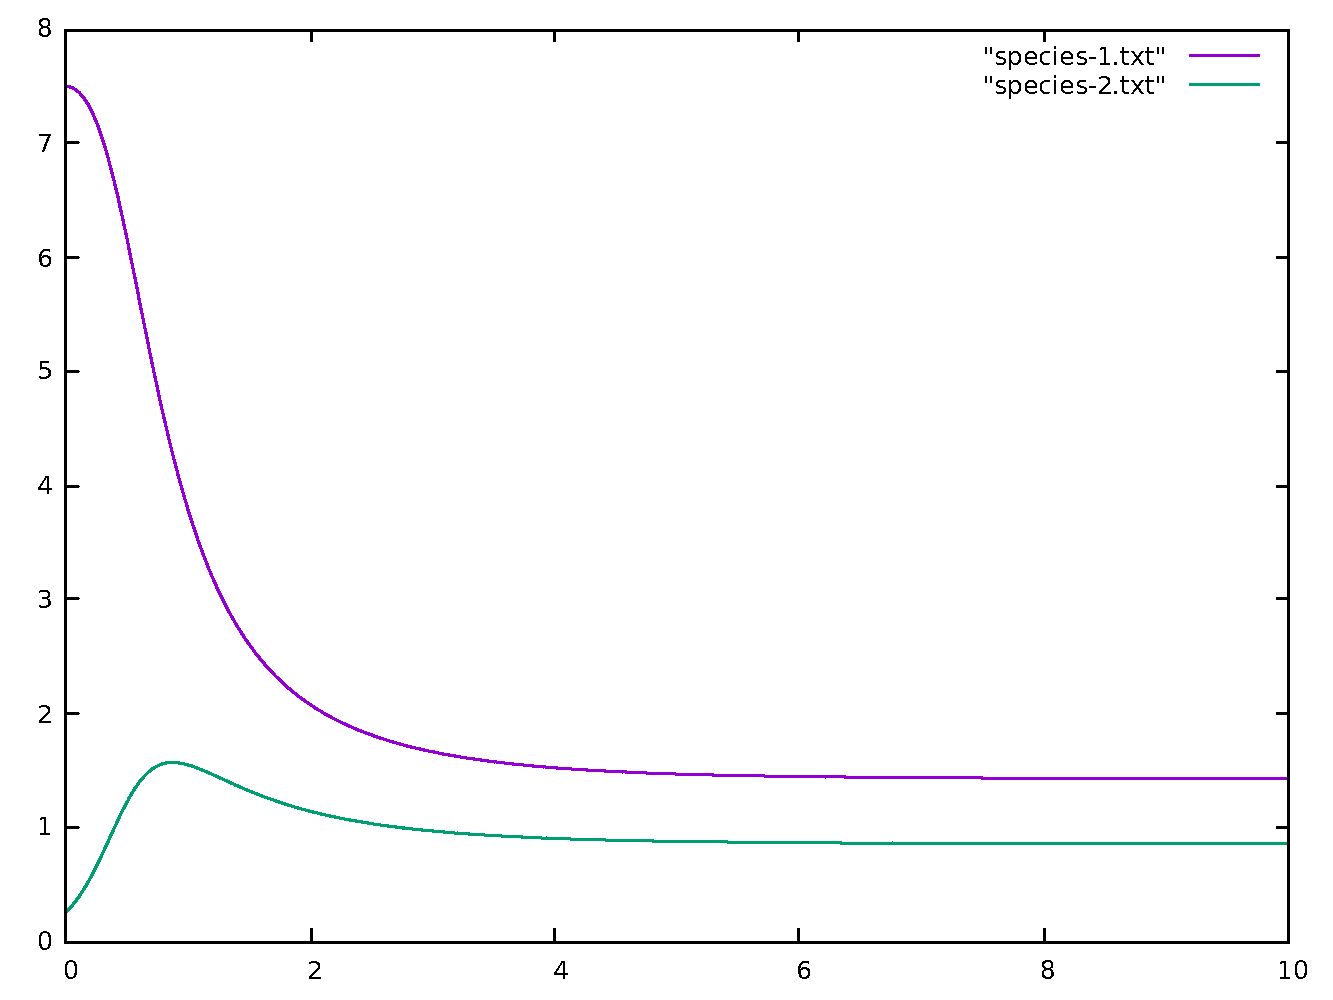
\includegraphics[height=9.25cm]{Figs/pokus_1}
\caption{$a=0.1$, $b=2$, $c=1$, $d=0.5$.}
\end{figure}

\begin{figure}[ht!]
\centering
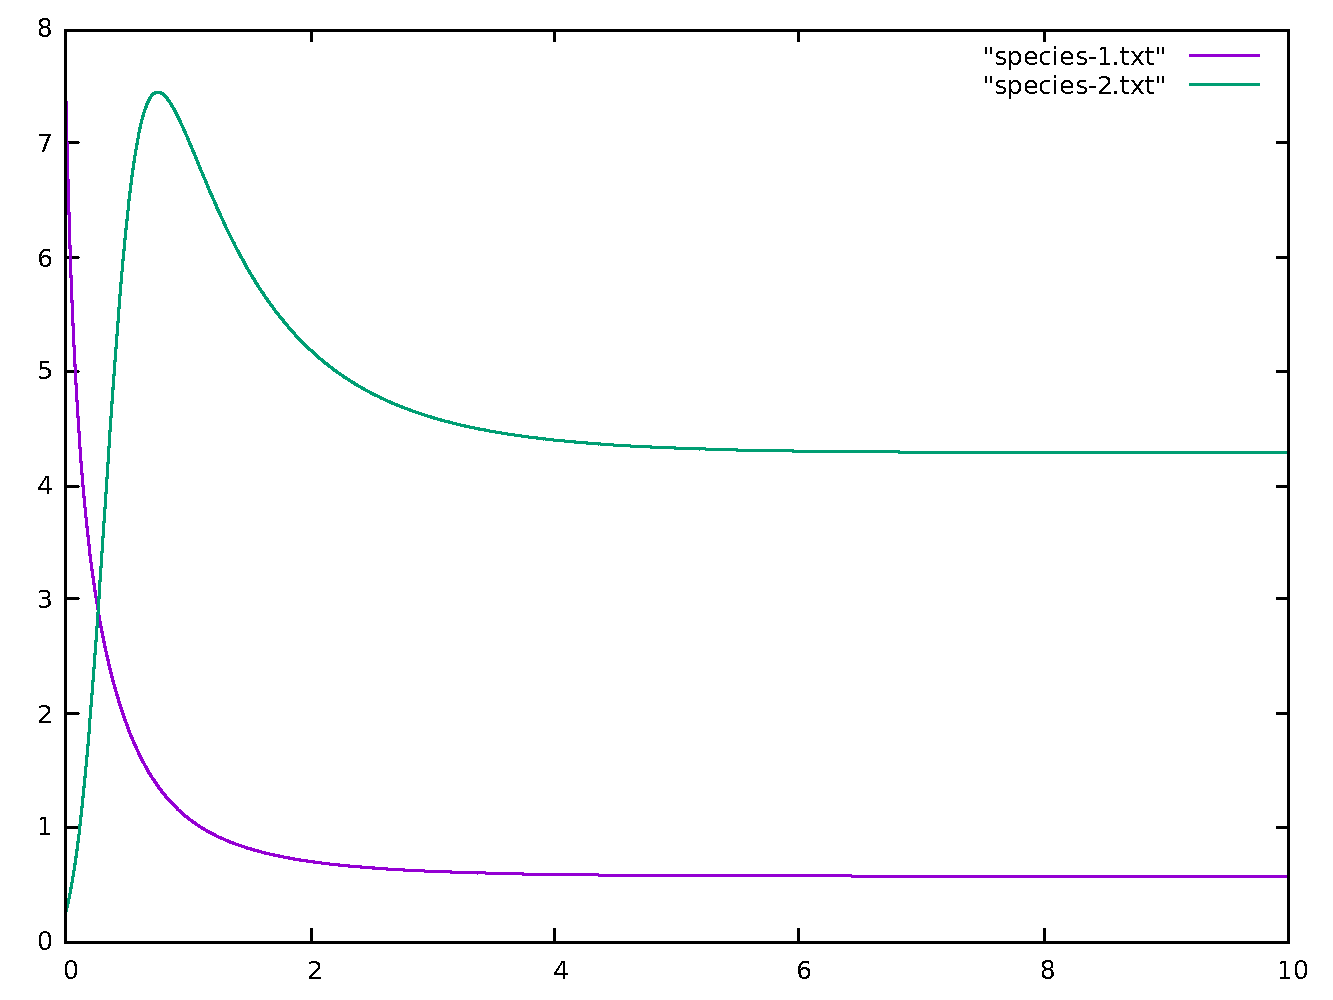
\includegraphics[height=9.25cm]{Figs/pokus_2}
\caption{$a=1$, $b=0.5$, $c=0.1$, $d=2$.}
\end{figure}

\end{document}
